\documentclass[conference,a4paper]{IEEEtran}
\usepackage{graphicx}
\usepackage{amsmath}
\usepackage{booktabs}
\usepackage{cite}
\usepackage{url}
\pagestyle{empty}

\newcommand{\refpending}{\textbf{[ref.\ pending]}}

\begin{document}

\title{AgriQ: An AI and Quantum-Inspired System for\\Smart Crop Planning under Land and Water Constraints}

\author{\IEEEauthorblockN{Anonymous Submission}
\IEEEauthorblockA{NGIA-QC 2026 --- Double-blind review}}

\maketitle
\thispagestyle{empty}

\begin{abstract}
We present AgriQ, a crop-planning system that couples machine learning with
quantum-inspired combinatorial optimisation, evaluated on 174 real parcels
(1{,}464~ha) in Jenin, Palestine. A Random Forest scores crop suitability, and
allocation is written as a 1{,}914-variable QUBO in which prices fall as total
production rises and irrigation water is priced. In a $2\times2$ benchmark of
two encodings (one-hot penalty, domain-wall) and two solvers (simulated
annealing, discrete simulated bifurcation) over 20 seeds at a common
wall-clock budget, encoding choice decides whether the quantum-inspired solver
works: domain-wall raises its profit by 152\%, after which the two solvers are
statistically indistinguishable, while annealing performs best with one-hot.
A myopic greedy plan loses money by flooding the market. Holding the water
budget fixed, restricted access to Oslo Area C land forgoes \$0.23--1.22M/yr
depending on market size, and irrigation water binds only when that land is
included.
\end{abstract}

\begin{IEEEkeywords}
quantum-inspired optimisation, simulated bifurcation, QUBO, domain-wall
encoding, crop planning, random forest
\end{IEEEkeywords}

\section{Introduction}

Agricultural systems must balance production against what markets can absorb.
When many farmers plant the same crop, the combined harvest depresses prices
and turns individually sensible choices into collective losses. Palestinian
farmers are exposed to this through fragmented land access, a large share of
smallholders, and limited access to forecasting tools; the northern West Bank
has seen a cucumber glut in 2021 and a tomato price collapse in 2025
\refpending. Avoiding such outcomes is an allocation problem: deciding how land
is divided among crops, given that each crop's price depends on how much of it
is grown in total.

Two further constraints shape allocation in Jenin governorate. Under the Oslo
interim framework, land is divided into Areas A and B, administered by the
Palestinian Authority, and Area C, under Israeli control, where Palestinian
cultivation is heavily restricted; 32.5\% of the agricultural parcel area in
our study lies in Area C. Irrigation draws on an agricultural water budget of
about 6.0~Mm$^3$/yr \refpending.

Allocating $P$ parcels among $C$ crops admits $C^P$ assignments and does not
decompose, because revenue depends on aggregate production. Written as a
quadratic unconstrained binary optimisation (QUBO) problem, it can be passed to
quantum-inspired solvers such as simulated bifurcation (SB)~\cite{goto2021},
which is derived from a quantum-mechanical model but runs classical dynamics
on conventional hardware. Doing so requires an \emph{encoding}: a
representation of each parcel's crop choice in binary variables together with
a way to enforce ``one crop per parcel''. This choice is usually treated as an
implementation detail. We find that it is not.

Our contributions are: (i) a $2\times2$ encoding-by-solver benchmark on a real
1{,}914-variable agricultural QUBO, showing that encoding determines whether
the quantum-inspired solver succeeds; (ii) a QUBO formulation with
market-clearing prices and priced irrigation water; (iii) a bounded estimate of
the agricultural cost of restricted Area C access under a fixed water budget;
and (iv) evaluation of every learned component against a trivial baseline,
including an LSTM that does not outperform persistence.

\section{Literature Review}

\subsection{AI-Based Crop Recommendation and Price Forecasting}

Random Forest, an ensemble method built on bagged decision trees, remains a
strong baseline for tabular agricultural data because it handles nonlinear,
heterogeneous features --- soil nutrients, pH, temperature, rainfall ---
without extensive preprocessing~\cite{breiman2001}. Dey et
al.~\cite{dey2024} reached classification accuracies above 99\% for crop
recommendation using XGBoost on soil and climatic features, but their pipeline
stops at suitability: with no forecasting or allocation stage, a crop flagged
suitable may still be a poor planting choice if the market is already
saturated. Saha et al.~\cite{saha2025} went further, combining satellite-based
land mapping, machine-learning crop recommendation and yield prediction (above
95\% accuracy), and irrigation control; their LSTM component, however,
forecasts healthy vegetation area rather than market prices, so it cannot
signal oversupply before it occurs.

Long Short-Term Memory networks~\cite{hochreiter1997} model long-range
temporal dependencies and are widely applied to agricultural price series.
Their benefit is sensitive to record length, and a governorate-level price
history offers only a few decades of annual observations per crop. Comparison
against simple forecasting baselines is therefore essential rather than
optional, and we evaluate our LSTM against persistence, autoregressive,
moving-average and trend models before any forecast is used.

\subsection{Optimization Approaches: From Classical Methods to Quantum-Inspired Algorithms}

Crop allocation has traditionally been posed as linear programming, but
recent work treats it as a nonlinear problem that integrates prediction and
market effects. Li et al.~\cite{li2025} combined simulated annealing with a
genetic algorithm (H-SAGA) across 34 plots in mountainous northern China,
feeding neural-network price forecasts into the optimizer and constraining
production by regional market-absorption capacity and total farm water
supply; H-SAGA achieved profit-increment ratios 5--10 percentage points above
standalone GA, SA, PSO and ACO. Hou et al.~\cite{hou2026} paired particle
swarm optimization with simulated annealing and Monte Carlo simulation
(PSO--SA--MCS), lowering prices when production exceeds demand, and raised
expected profit by 12.6\% over a baseline PSO at a runtime complexity of
$O(N^2\cdot\mathrm{pop})$. Integrating forecasting, market saturation and
resource limits into one allocation model is thus established with classical
metaheuristics.

Quantum and quantum-inspired approaches offer a different route. Simulated
bifurcation (SB)~\cite{goto2021} is derived from a quantum-mechanical model
but simulates \emph{classical} Hamiltonian dynamics, so it runs on
conventional hardware. Zeng et al.~\cite{zeng2024} benchmarked
quantum-annealing-inspired algorithms, including SB variants, against a D-Wave
quantum annealer on Max-Cut instances with up to 20{,}000 nodes: ballistic SB
cut time-to-solution nearly fifty-fold relative to quantum annealing on small
and Chimera-structured graphs, and discrete SB reached targets fastest on large
graphs. On dense QUBO instances, Kim et al.~\cite{kim2025} found a hybrid
quantum-annealing solver roughly 6{,}561$\times$ faster than the best
classical solver, with marginally higher accuracy. In agriculture, Verma et
al.~\cite{verma2025} proposed HQOMLF, combining a quantum convolutional neural
network for prediction with the Quantum Approximate Optimization Algorithm for
resource allocation, and reported speed-ups of up to 3.5$\times$.

Two points remain unaddressed. First, none of these agricultural studies
formulates allocation as a QUBO with market-clearing prices for Ising-type
solvers: Li et al.\ and Hou et al.\ use classical metaheuristics, and Verma et
al.\ apply QAOA without a market model. Second, the benchmarking literature
compares \emph{solvers}, yet on a real problem results also depend on how
constraints are \emph{encoded}. The standard one-hot encoding enforces one
crop per parcel through a penalty, leaving invalid assignments reachable;
Chancellor's domain-wall encoding~\cite{chancellor2019} makes them
unreachable by construction. Whether encoding matters as much as solver choice
on a real allocation problem has not, to our knowledge, been measured.
Table~\ref{tab:lit} summarizes the studies reviewed.

\begin{table*}[t]
\centering
\caption{Summary of reviewed studies across crop recommendation, forecasting, and optimization}
\label{tab:lit}
\footnotesize
\begin{tabular}{p{2.6cm}p{3.3cm}p{4.2cm}p{6.2cm}}
\toprule
Study & Focus area & Method & Limitation relative to this study \\
\midrule
Breiman~\cite{breiman2001} & Ensemble learning, general & Random Forest (foundational) & Not agricultural; establishes the method applied here to crop suitability \\
Hochreiter \& Schmidhuber~\cite{hochreiter1997} & Sequence modeling, general & LSTM (foundational) & Not agricultural; establishes the method applied here to price forecasting \\
Dey et al.~\cite{dey2024} & Crop recommendation & XGBoost on soil/climate features & Suitability only; no forecasting or allocation stage \\
Saha et al.~\cite{saha2025} & Land suitability, irrigation & ML + LSTM (vegetation), satellite data & LSTM forecasts vegetation area, not prices; no allocation across parcels \\
Li et al.~\cite{li2025} & Dynamic multi-plot crop planning & Hybrid SA--GA + neural-network price forecasts & Classical metaheuristic; no QUBO formulation or encoding analysis; no land-access restrictions \\
Hou et al.~\cite{hou2026} & Crop planning under uncertainty & Hybrid PSO--SA + Monte Carlo & No learned forecasts; classical metaheuristic; $O(N^2\cdot\mathrm{pop})$ runtime \\
Zeng et al.~\cite{zeng2024} & Quantum-inspired optimization & SB and simulated CIM vs.\ D-Wave annealer & Abstract Max-Cut benchmarks; compares solvers, not encodings \\
Kim et al.~\cite{kim2025} & Large-scale dense QUBO & Hybrid quantum annealing vs.\ classical solvers & Benchmark instances, not agricultural; compares solvers, not encodings \\
Verma et al.~\cite{verma2025} & Quantum computing in precision agriculture & QCNN + QAOA (HQOMLF) & No market-clearing prices; no QUBO encoding analysis; no comparison with SB \\
Chancellor~\cite{chancellor2019} & Encoding discrete variables & Domain-wall encoding & Theoretical; not evaluated on a real-world allocation problem \\
\bottomrule
\end{tabular}
\end{table*}

Taken together, integrated crop planning that combines prediction, market
saturation and resource limits is established with classical
metaheuristics~\cite{li2025,hou2026}, and quantum-inspired solvers perform
strongly on abstract benchmarks~\cite{zeng2024,kim2025}. What has not been
examined is where the two meet: agricultural allocation written as a QUBO with
market-clearing prices, and the effect of constraint encoding on the solvers
that consume it. This study addresses that gap on 174 real parcels in Jenin,
while accounting for the land-access and water constraints specific to the
Palestinian context.

%% ============================================================
%% METHODOLOGY -- REMOVED, TO BE WRITTEN BY TALA
%% The removed text is preserved in METHODOLOGY_REMOVED.tex
%% See METHODOLOGY_BRIEF.md for the numbers it must report.
%% ============================================================
\section{Methodology}

[To be written.]

\section{Results}

\subsection{Suitability and Price Forecasting}

In 5-fold stratified cross-validation, the Random Forest reaches
$0.9945\pm0.0037$ accuracy on real data against a majority-class baseline of
0.0455. On synthetic EcoCrop rows it reaches $0.8514\pm0.0291$, which measures
fidelity to the envelopes rather than predictive skill. Feature importances are
rainfall 0.251, humidity 0.192, K 0.166, P 0.139, N 0.098, temperature 0.082
and pH 0.072, so the unmeasured P and K carry 30.5\%. Under Jenin's inputs the
model gives oranges zero probability on every parcel, so oranges are never
assigned.

An LSTM~\cite{hochreiter1997} (24 hidden units, 3{,}481 parameters) was trained
on pooled log-price windows with augmentation applied to training data only,
under walk-forward validation with the split made before normalisation
(Table~\ref{tab:lstm}).

\begin{table}[t]
\centering
\caption{Price forecasts, 50 test windows, 2024 excluded}
\label{tab:lstm}
\footnotesize
\begin{tabular}{lcc}
\toprule
Model & RMSE (\$/t) & MAPE (\%) \\
\midrule
\textbf{Persistence} & \textbf{130.1} & \textbf{16.3} \\
AR(1) & 150.5 & 18.3 \\
Mean of last 3 & 170.1 & 19.7 \\
Linear trend & 186.0 & 20.9 \\
LSTM (pooled, augmented) & 252.2 & 26.7 \\
\bottomrule
\end{tabular}
\end{table}

The LSTM ranks last. With 142 training windows from 13--27 annual observations
per crop, 3{,}481 parameters are not constrained, and augmentation adds no
information. The optimisation therefore uses the 2019--2023 mean prices. When
2024 is included in the test window, the ranking reverses (LSTM RMSE 624.2
against 639.6 for persistence). The wartime shock raises persistence error
4.9-fold but LSTM error only 2.5-fold, so a test window containing 2024
rewards robustness to a discontinuity rather than forecasting skill.

\subsection{Encoding Versus Solver}

\begin{table}[t]
\centering
\caption{Encoding by solver, 20 seeds, 2.5\,s per run}
\label{tab:bench}
\footnotesize
\setlength{\tabcolsep}{4pt}
\begin{tabular}{llcccc}
\toprule
Enc. & Solver & Profit (M\$) & Invalid & Unsuit. & Water (Mm$^3$) \\
\midrule
one-hot & SA  & $5.42\pm0.26$ & 0.0   & 0.5  & 5.48 \\
one-hot & dSB & $1.98\pm0.42$ & 129.1 & 10.7 & 2.20 \\
dom.-wall & SA  & $4.97\pm0.39$ & 13.0 & 0.3 & 6.25 \\
dom.-wall & dSB & $5.00\pm0.30$ & 2.9  & 0.0 & 5.97 \\
\midrule
\multicolumn{2}{l}{Greedy} & $-1.58$ & --- & 0 & 5.98 \\
\bottomrule
\end{tabular}
\end{table}

\begin{figure}[t]
\centering
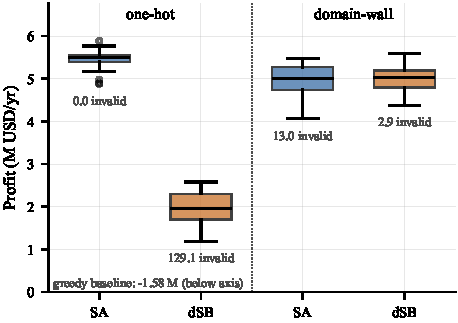
\includegraphics[width=\columnwidth]{figures/fig_encoding.pdf}
\caption{Profit over 20 seeds, with the mean number of parcels holding an
invalid assignment.}
\label{fig:encoding}
\end{figure}

Table~\ref{tab:bench} and Fig.~\ref{fig:encoding} give the results; ``Invalid''
counts parcels whose binary block is not a valid assignment. With one-hot
encoding, dSB leaves 129 of 174 parcels invalid and earns 63\% less than SA
($p<10^{-7}$). Its continuous dynamics bifurcate variables independently, and
the dense per-parcel penalty does not reliably leave exactly one positive.
Domain-wall encoding raises dSB profit by 152\% ($p<10^{-7}$), and the two
solvers then do not differ (dSB $+0.6\%$, $p=0.93$). The encoding effect is
not symmetric: domain-wall \emph{lowers} SA profit by 8.5\% ($p<10^{-4}$) and
leaves SA with 13 invalid parcels, because the ordering penalty is not sized
to SA's single-bit moves. The best configuration is therefore classical SA
with one-hot encoding. The finding is that encoding choice decides whether the
quantum-inspired solver is usable, not that it outperforms annealing.

The greedy plan loses \$1.58M. Assigning every parcel its best-margin crop
concentrates production in a few crops far beyond $D_j$. Even if unsaleable
surplus is discarded rather than sold at the negative prices a linear demand
curve implies beyond $2D_j$, it still loses \$1.55M. This is the glut
mechanism that motivates the study.

\subsection{Water Shadow Price and Area C Access}

\begin{figure}[t]
\centering
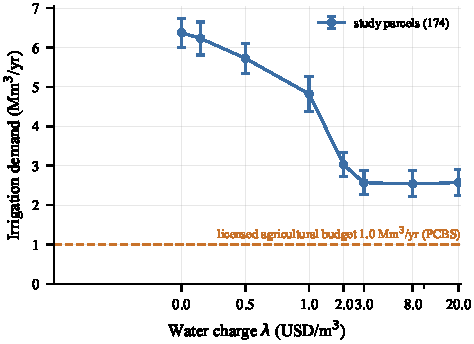
\includegraphics[width=\columnwidth]{figures/fig_water.pdf}
\caption{Irrigation demand against the water charge $\lambda$ (SA, one-hot,
10 seeds; bars are one standard deviation).}
\label{fig:water}
\end{figure}

Sweeping $\lambda$ traces the demand for irrigation water
(Fig.~\ref{fig:water}). On Areas A/B, demand peaks at 5.50~Mm$^3$/yr, so the
6.0~Mm$^3$ budget never binds and its shadow price is zero. With Area C and
the same market, demand reaches 7.96~Mm$^3$ and the budget binds at
\$1.09/m$^3$; if the market grows with land, the shadow price is \$1.35/m$^3$.

\begin{table}[t]
\centering
\caption{Area C counterfactual within the 6.0\,Mm$^3$ water budget}
\label{tab:areac}
\footnotesize
\setlength{\tabcolsep}{4pt}
\begin{tabular}{lccc}
\toprule
Regime & Area (ha) & Profit (M\$/yr) & Forgone \\
\midrule
Areas A/B & 1{,}464 & 5.36 & --- \\
A/B + C, market fixed & 2{,}169 & 5.59 & 0.23 \\
A/B + C, market $\times1.48$ & 2{,}169 & 6.58 & 1.22 \\
\bottomrule
\end{tabular}
\end{table}

Table~\ref{tab:areac} compares land regimes at the same prices, yields,
suitability thresholds and water budget. Withholding 706~ha of Area C land
forgoes \$0.23M/yr if the market is limited to its present size, and
\$1.22M/yr if Area C access brought proportionate market access. The range is
wide because, with water binding and a fixed market, additional land mostly
adds supply that cannot be sold at a profit; the value of land access depends
on market access. On SoilGrids estimates, Area C and A/B parcels are similar in
pH (7.69 vs.\ 7.71), clay (46.2 vs.\ 46.4\%) and cation exchange capacity (34.2
vs.\ 36.0~cmol/kg), and Area C has higher soil organic carbon (28.3 vs.\
20.7~g/kg); these estimates give no indication that Area C land is poorer.

\subsection{Price Robustness}

The optimum is degenerate: inverse demand equalises marginal revenue across
crops, so many parcel-level plans reach similar profit, and two baseline runs
differing only in seed agree on just 18.4\% of parcels. We therefore compare
crop mix by area, as $1-$ total variation distance, against a seed-control
floor (10 seeds each).

\begin{table}[t]
\centering
\caption{Crop-mix similarity to the baseline plan}
\label{tab:robust}
\footnotesize
\begin{tabular}{lcc}
\toprule
Scenario & Profit (M\$/yr) & Mix similarity \\
\midrule
\emph{Seed control} & \emph{5.12} & \emph{93.0\%} \\
LSTM prices / persistence & 4.96 / 4.93 & 93.0 / 93.7\% \\
Uniform $-15\%$ / $+15\%$ & 3.20 / 7.41 & 90.6 / 93.2\% \\
Uniform $+30\%$ / perish.\ $+30\%$ & 9.80 / 8.86 & 91.6 / 92.1\% \\
Uniform $-30\%$ / perish.\ $-30\%$ & 1.45 / 2.38 & 84.6 / 84.4\% \\
\bottomrule
\end{tabular}
\end{table}

All moderate scenarios, including the LSTM and persistence price vectors,
lie within 2.4 points of the seed-control floor. Only a 30\% price fall shifts the crop mix
beyond that, moving land toward grapes, olives, wheat and fallow.

\section{Limitations}

Market size $D_j$ is an assumption, and the Area C result is bounded rather
than estimated for that reason. The linear demand curve is not meaningful
beyond $Q_j=2D_j$. Climate is a single grid cell; phosphorus and potassium are
sampled; available nitrogen and irrigation requirements are approximations;
and SoilGrids values are model estimates, not field measurements. Yields are
national series rescaled to regional open-field levels, and tree crops are
assumed to be at steady bearing. The domain-wall ordering penalty was not
tuned, which leaves invalid parcels under SA. OpenStreetMap under-represents
unmapped smallholdings. At 1{,}914 variables with ten 174-node crop cliques,
the instance also exceeds the largest fully connected problem that can be
directly embedded on current annealing hardware ($K_{150}$ on
Pegasus~\cite{dwaveembed}), although hybrid quantum--classical
solvers~\cite{kim2025} could accept it.

\section{Conclusion}

On a real 1{,}914-variable crop-allocation QUBO, encoding choice decided
whether a quantum-inspired solver was usable. Domain-wall encoding raised
discrete simulated bifurcation's profit by 152\%, bringing it level with
simulated annealing, although annealing with one-hot encoding remained the
best configuration. A myopic greedy plan lost money by flooding the market,
which is what market-aware allocation is meant to prevent. For Jenin,
irrigation water does not bind on the land farmers can currently use, and
access to Area C land is worth \$0.23--1.22M/yr within the water budget
depending on market access. Future work should tune the domain-wall penalty,
obtain crop-level demand data, and extend the model to multi-season rotations.

\bibliographystyle{IEEEtran}
\bibliography{references}

\end{document}
